\documentclass{tccv}
\usepackage[english]{babel}
\usepackage{graphicx}
\usepackage{epigraph}

\begin{document}

\part{\href{https://scholar.google.ca/citations?view_op=list_works&hl=en&user=WHhfJSMAAAAJ}{Anubhav Chaturvedi}}

\personal
    {Kujawska 48\newline 81-828 -- Sopot, Poland}
    {+48 533751991}
    {anubhav.chaturvedi@research.iiit.ac.in}

\section{Research Interests}
\begin{itemize} \itemsep -0pt %\renewcommand{\labelitemi}{$\star$}
\item Foundations of quantum mechanics.
\item Query and communication complexity.
\end{itemize}




\section{Education}

\begin{yearlist}
\item[Master studies]{2014 -- 2016}
     {M.S. by Research in Computational Natural Sciences (CNS)}
     {International Institute of Information Technology, Hyderabad, India}

\item[Bachelor studies]{2010 -- 2014}
     {Bachelor of Technology (Honours) in Computer Science (CSE)}
     {International Institute of Information Technology, Hyderabad, India}
\end{yearlist}

\section{Publications}

\begin{yearlist}
\item{2018}
{\href{https://link.springer.com/article/10.1007/s11128-018-1892-z}{On the security of semi-device-independent QKD protocols}}{\textsc{A. Chaturvedi, M. Ray, R. Veynar, M. Paw{\l}owski.} Quantum Inf Process. VOL. 17, NO. 131.}

\item{2017}
{\href{https://journals.aps.org/pra/abstract/10.1103/PhysRevA.96.022125}{Random access codes and nonlocal resources
}}{\textsc{A. Chaturvedi, M. Paw{\l}owski, K. Horodecki.} Phys. Rev. A VOL. 96, NO. 022125.}

\item{2017}
{\href{https://journals.aps.org/pra/abstract/10.1103/PhysRevA.96.022121}{Complementarity of genuine multipartite Bell nonlocality}}{\textsc{S. Sami, I. Chakrabarty, A. Chaturvedi.} Phys. Rev. A VOL. 96, NO. 022121.}
\item{2015}
{\href{http://iopscience.iop.org/article/10.1209/0295-5075/112/30003}{Measurement-device-independent randomness from local entangled states.}}{\textsc{A. Chaturvedi, M. Banik.}  EPL (Europhysics Letters), VOL. 112, NO. 3.}

\item{2013}
{\href{http://www.currentscience.ac.in/Volumes/105/09/1275.pdf}{Application of fractal geometry in determining optimal quadrat size for vegetation sampling.}}{\textsc{A. Chaturvedi, R. C. Prasad.}  CURRENT SCIENCE, VOL. 105, NO. 9.}


\end{yearlist}

\section{Preprints}

\begin{yearlist}
     
\item{2018}
{\href{https://arxiv.org/abs/1802.07215}{Preparation contextuality: the ground of quantum communication advantage}}{\textsc{D. Saha, A. Chaturvedi.} arXiv:1802.07215. In communication with Phys. Rev. Lett.}

\item{2016}
{\href{http://arxiv.org/abs/1603.09120}{ Parity Oblivious d-Level Random Access Codes and A Class of Non-contextual Inequalities}}{\textsc{A. Ambainis, M. Banik, A. Chaturvedi, D. Kravchenko, A. Rai.} arXiv:1607.05490. In communication with Quantum Inf Process. }

\end{yearlist}

\section{On-going projects}
\begin{yearlist}
    \item{} 
    {Unified framework for communication and correlations}{Collaborators: D. Saha, P. Mironowicz, M. Paw{\l}owski}
    \item{} 
    {Application of contextuality in semi device independent setting.}{Collaborators: D. Saha, A. Tavakoli, M. Paw{\l}owski}
    \item{}
    {The ontic-feature underlying all finite dimensional quantum advantage}{Collaborators: D. Saha, M. Oszmaniec}
    \item{}
    {Comparing assignment and discard strategies for dealing with detection efficiency loophole}{Collaborators: N. Miklin, M. Paw{\l}owski}
    \item{}
     {Symmetrisation of linear programming and applications in quantum information.}
     {Collaborators: N. Miklin}
    
\end{yearlist}

\section{Research Positions}

\begin{yearlist}
\item{2016 - 2018}{Research Assistant, National Quantum Information Centre in Gdansk, Poland.}{Supervisor: Dr. M. Paw{\l}owski}

\item{2014}{Summer Research Intern, National Quantum Information Centre in Gdansk, Poland.}{Supervisor: Dr. M. Paw{\l}owski}

\item{2013}{Summer Research Intern, Physics and Applied Mathematics Unit, Indian Statistical Institute, Kolkata, India.}{Guide: Prof. G. Kar}

\end{yearlist}

\section{Teaching Positions}

\begin{yearlist}
\item{2015}{Teaching Assistant: Science I.}{Guide: Prof. P. Bhimalapuram}

\item{2014}{Teaching Assistant: Quantum Mechanics, Symmetry and Spectroscopy.}{Lecturer: Prof. H. Singh}

\item{2014}{Teaching Assistant: Science II.}{Lecturer: Prof. P. Bhimalapuram}

\item{2013}{Teaching Assistant: Mathematics I (Discrete Mathematics).}{Lecturer: Prof. I. Chakrabarty}

\end{yearlist}
\section{Poster presentations}

\begin{yearlist}
\item{2018}{Quantum Information Workshop Seefeld.}{Organised by University of Innsbruck, Austria.}
\item{2017}{International Conference for “Young Quantum Information Scientists”.}{Organised by the Max Planck Institute for the Science of Light, Erlangen, Germany.}
\item{2017}{Foundations of Quantum Mechanics and Technology (FQMT)}
{Organised by International Centre for Mathematical Modelling in physics, engineering and cognitive sciences (ICMM) at Linnaeus University in Vaxjo, Sweden.}
\item{2015}{QUANTUM CORRELATION; Foundation, Information Processing and Various Applications.}{Organized by Physics and Applied Mathematics Unit, Indian Statistical Institute, Kolkata, India.}
\item{2013}{QCrypt: 3rd international conference on quantum cryptography}{Organised by Institute for Quantum Computing, Waterloo, Canada.}
\item{2013}{Asian Quantum Information Science Conference (AQIS)}{Organized
by the Institute of Mathematical Sciences Taramani, Chennai, India.
}
\end{yearlist}



\\
\vspace{4in}
\section{Awards}

\begin{yearlist}

\item{2012-2013}{Dean's Research List.}{Recommended by: Dr. R. C. Prasad and Dr. I. Chakrabarty. One of the most prestigious awards at International Institute of Information Technology, Hyderabad, India. The first undergraduate to receive it.}
\item{2009-2010}{National Talent Search Scholarship.}{Scholarship for talent in academics: Physics, Mathematics.}

\end{yearlist}

\section{Software skills}

\begin{factlist}

\item{Programming}
     {C, C++, Python, Bash Scripting.}

%\item{Graphics}
%     {OpenGL}

\item{Web Development}
     {HTML/CSS, JavaScript, AJAX.}
     
\item{Databases}
	 {MySQL, sqlite.}
     
\item{Typesetting / Publishing}
	 {\LaTeX.}
 
\item{Mathematical Tools}
	 {Mathematica, MATLAB, Octave. }
     
\item{Platform(s)}
	 {Linux (Fedora, Ubuntu, Debian).}

\end{factlist}
\section{Cited by}
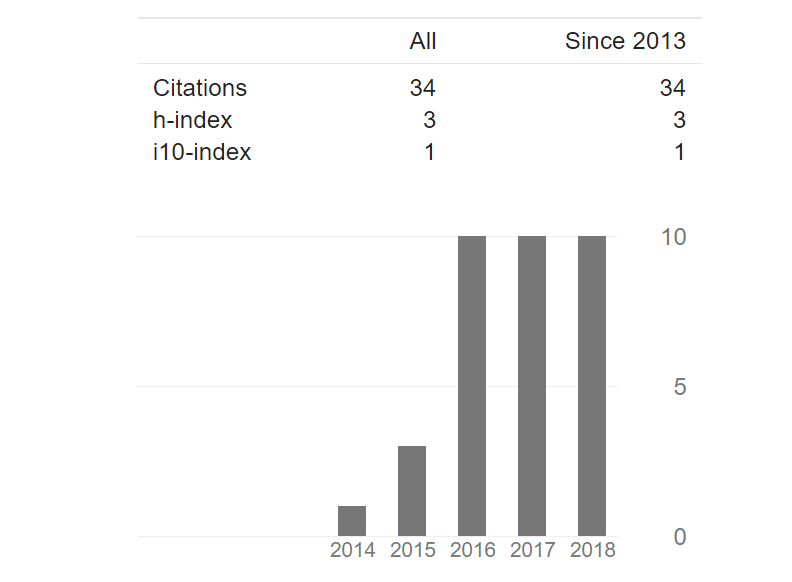
\includegraphics[scale=0.5]{citations.png}
\vspace{1.5in}
\epigraph{Ultimately, all moments are really one, therefore now is an eternity.}{\textit{David Bohm}}

\end{document}
